% 记录阅读文献时遇到的一些数学概念等
\subsection{采样}
采样是生成一堆数据的过程, 如果最终生成的数据服从某个分布, 则可以称这堆数据采样自这个分布. 
\subsubsection{alias sampling }
一种高效的针对\textbf{离散概率分布}采样方法, 但是要先经过预处理, 预处理的时间为$O(n)$, 但是与处理完成后采样的时间时$O(1)$. 预处理的大致思路如下: \\
对于一个给定的离散概率分布: $p(X = x_i) , X = x_1, x_2, ..., x_n$. 按照序号构造n个盒子, 每个盒子按照顺序一一与$x_1, ..., x_n$对应, 每个盒子的高度为$n \cdot p(X = x_i)$. 接下来通过取长补短, 把高度高于1的盒子切一部分分到其他高度低于1的盒子上, 而且每个序号对应处不能有超过两个盒子. 所以需要两个数组(Alias, Accept)来记录预处理的结果, 一个用来记录每个序号除了原来的盒子还放了哪个盒子, 一个用来记录每个序号的外来盒子有多高. \\
进行采样时, 先决定使用哪个序号对应的盒子, 再决定使用该序号内的原来的盒子还是外来的盒子. 一个简单的例子Fig.\ref{fig:alias-sample}
\begin{figure}[h]
	\centering
	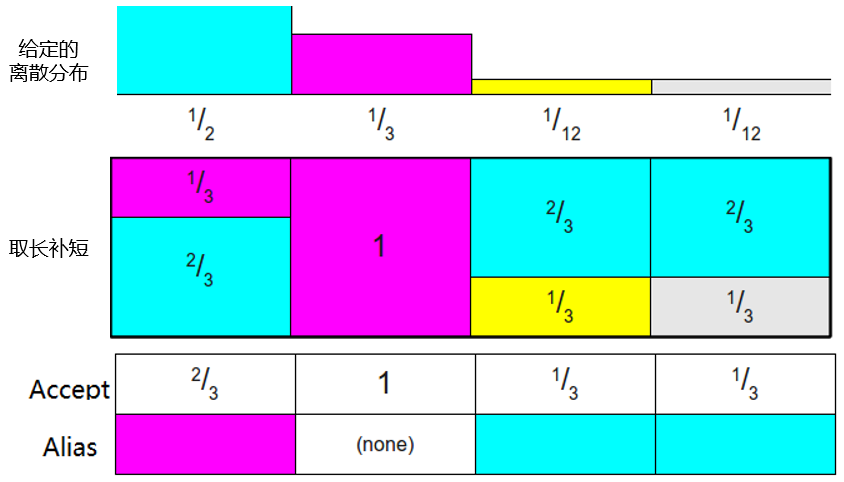
\includegraphics[width=.8\textwidth]{pics/alias-sample.png}
	\label{fig:alias-sample}
	\caption{Alias Sample例子}
\end{figure}


参考资料: 
\begin{enumerate}
    \item \href{https://www.keithschwarz.com/darts-dice-coins/}{Darts, Dice, and Coins: Sampling from a Discrete Distribution}
    \item \href{https://www.cnblogs.com/dogecheng/p/13198198.html}{【图嵌入】DeepWalk 和 Node2Vec}
\end{enumerate}

\subsubsection{Importance Sampling}
重要性采样, 一种近似的抽样方法, 通过一些数学上的变化, 使得可以对一些不好抽样的分布进行抽样和估计. 这个会在强化学习中的off-policy的方法中用到, 从一个策略进行抽样, 更新另外一个策略. 求函数$f(x)$的积分可以写成求期望的形式: 
$$
E_{x \sim p(x)}[f(x)] = \int p(x) f(x) d x \approx \frac{1}{n} \sum_{i} f(x_{i})
$$
然而通常数据分布会比较复杂且积分也是一个复杂的过程, 因此会用采样来代替之. 上式中的第三项就是用采样来代替积分, 其中$\frac{1}{n}$表示$p(x) = \frac{1}{n}$, 即数据的分布. 但是有时候$p(x)$是个很复杂的分布, 从其重采样是很困难的, 这个时候该怎么办呢?

找一个易于采样的分布$q(x)$, 如正态分布, 从$q(x)$中采样得到的很多样本作为从$p(x)$中采样的样本集, 那么问题就来了, 这俩又不是同一个分布, $q(x)$中采样的样本集分布符合$p(x)$吗?先看一个公式: 
$$
E_{x \sim p(x)}[f(x)] = \int q(x) \frac{p(x)}{q(x)} f(x) d x \approx \frac{1}{n} \sum_{i}  \frac{p(x)}{q(x)} f(x_{i})
$$
这个就是当我们从$q(x)$中采样代替$p(x)$后求$f(x)$积分/期望的公式. 可以看出对于从$q(x)$中采样的样本赋予了不同的权重, 因为样本集来自$p(x)$的概率是不一样的, 其中重要性就是$\frac{p(x)}{q(x)}$. 如Fig.\ref{fig:importance-sample}所示. 注意: 图中$p(z)$与$f(z)$的含义, $p(z)$是一种分布, 是相对于$z$轴的采样点而言的, 比如在红色的两个驼峰处, $z$的取点比较多, 在其他地方$z$的取点就比较少, 这叫样本分布服从$p(z)$. 对于$f(z)$是一种映射关系, 将$z$值映射到其他维度. 

\begin{figure}[h]
	\centering
	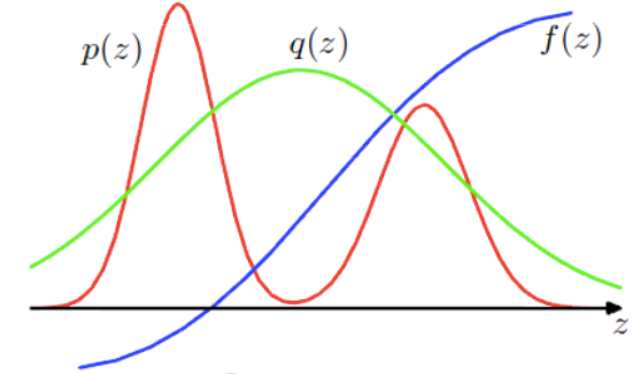
\includegraphics[width=.5\textwidth]{pics/importance-sample.png}
	\label{fig:importance-sample}
	\caption{重要性采样}
\end{figure}

参考: \href{https://www.jianshu.com/p/3d30070932a8}{随机模拟-Monte Carlo积分及采样(详述直接采样、接受-拒绝采样、重要性采样)}. 


\subsubsection{接受-拒绝采样}
同样的问题: 对于一个难以采样的分布$p(x)$, 该怎么采样呢?选择一个易于采样的分布$q(x)$, 从中采样, 以一定的概率接受或拒绝采样到的样本, 使得经过筛选后的样本集是服从$p(x)$的. 
\begin{figure}[h]
	\centering
	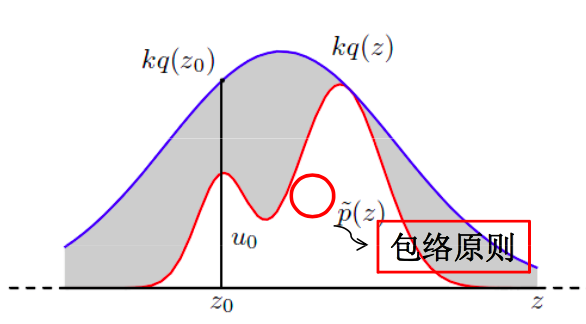
\includegraphics[width=.6\textwidth]{pics/accept-reject-sample.png}
	\label{fig:accept-reject-sample}
	\caption{接受-拒绝采样}
\end{figure}
具体该怎么操作呢?如Fig.\ref{fig:accept-reject-sample}所示, 选择$q(x)$, 乘以$k$得到$kq(x)$使之刚好能够包住$p(x)$. 对于$q(x)$中采样到的样本$z_0$, 从$[0, 1]$的均匀分布中取一个数$u_0$, 如果$u_0 \le \frac{p(z_0)}{q(z_0)}$则接受$z_0$. 

\subsubsection{蓄水池抽样}
主要解决的问题: \textbf{给定一个数据流, 数据流长度 $N$ 很大, 且在数据处理完之前 $N$ 都是未可知的, 请问如何在只遍历一遍数据的情况下, 随机选出 $k$ 个数据, 使每个元素被抽到的概率相等}.

\textbf{抽样过程}:
\begin{enumerate}
	\item 构建一个可容纳 $k$ 个元素的数组 (即蓄水池) $nums$;
	
	\item 读取数据流的第 $i$ (从 1 开始) 个元素, 若 $i \leq k$ 则将其直接放入数组;
	
	\item 当 $i > k$ 时, 在 $[0, i-1]$ 内选去随机数 $d$, 若 d 小于 $k$ 则用第 $i$ 个数据替换 $nums[d]$. \textcolor{red}{第 $i$ 个元素进入蓄水池的概率是 $\frac{k}{i}$};
	
	\item 遍历完所有元素后得到最终的抽样结果.
\end{enumerate}

\textbf{证明}:由于要求每个元素被抽到的概率是相等的,那么每个数据最后保留下来的概率应该等于 $\frac{k}{N}$ --- 这就是证明的目标. 

对于数据流中前 $k$ 个数据, 首先会被保留在蓄水池中, 当读取第 $k+1$ 个元素时, 我们来计算蓄水池中第 $i$ 个元素被替换的概率. 被第 $k+1$ 个元素替换的概率 = 第 $k+1$ 个元素被选中的概率 * $i$ 被选中的概率, 即 $\frac{k}{k+1} \times \frac{1}{k}$. 那么 $nums[i]$ 不被第 $k+1$ 个元素替换的概率未 $1 - \frac{1}{k+1}$. 依此类推, 则\textcolor{red}{运行至第 $N$ 步时, $nums[i]$ 还没被替换的概率}未:

$$
1 \times \frac{k}{k+1} \times \frac{k+1}{k+2} \times \frac{k+2}{k+3} \times \dots \times \frac{N-1}{N} = \frac{k}{N}
$$

对于数据流中的第 $j$ ($j > k$) 个数. 其在第 $j$ 步被选中的概率为 $\frac{k}{j}$, 不在第 $j+1$ 步被替换的概率为 $1 - \frac{k}{j+1} \times \frac{1}{k} = \frac{j}{j+1}$. 依此类推, 则 \textcolor{red}{运行至第 $N$ 步时, 保留下来的概率为}:

$$
\frac{k}{j} \times \frac{j}{j+1} \times \frac{j+1}{j+2} \times \dots \times \frac{N-1}{N} = \frac{k}{N}
$$

综上所述, 对于数据流中的 $N$ 个元素, 每个元素被保留下来的概率为 $\frac{k}{N}$.


\subsection{eigen-value \& eigen—vector }
特征值, 特征向量. 
这两者到底有什么意义呢?


\subsection{Density estimation }

\subsection{MMD}
Maximum mean discrepancy.  用来衡量两个分布的差异. 具体的衡量过程是: 
假设有两个分布p, q, 那么利用这两个分布分别生成两个样本集ps, qs, 再假设有一个函数f, 对于$pm = \sum_{i \in ps}f(i), qm = \sum_{j \in qs}f(j) $,
则分布p, q 在f上的MMD为 $pm$与$qm$的差或某种基于$pm, qm$ 的计算值. 

\subsection{P, NP, NP-hard}
P问题: 确定性计算机能够在指数级时间解决的问题;

NP问题: 非确定性计算机能够在指数级时间解决的问题;

NPC问题: 存在这样一个NP问题, 所有NP问题都能约化成它, 即只要解决了这个问题则所有NP问题都能解决. NPC需要满足两个条件: 
\begin{itemize}
	\item 它是一个NP问题
	\item 所有的NP问题都能规约到它
\end{itemize}

NP-hard问题: 满足NPC问题的第二个条件, 但不一定满足第一条. NP-hard问题同样难以找到多项式时间的解法, 但不一定是NP问题. 这几者之间的包含关系如\ref{fig:P-NP-NPC-NP-hard}所示. 

\begin{figure}[h]
	\centering
	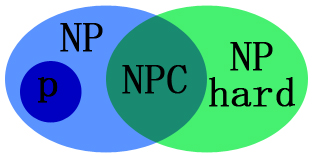
\includegraphics[width=.4\textwidth]{pics/P-NP-NPC-NP-hard.jpeg}
	\caption{P\_NP\_NPC\_NP-hard}
	\label{fig:P-NP-NPC-NP-hard}
\end{figure}



\subsection{傅里叶变换和小波分析}
傅里叶变换: 知道一段时间内, 信号的各个频率分量分别有多少. 
小波变换: 知道一段时间内, 信号的各个频率分量分别有多少, 以及它们都是什么时候出现的. 

参考资料: \href{https://cseweb.ucsd.edu/~baden/Doc/wavelets/polikar_wavelets.pdf}{《The Wavelet Tutorial》}、\href{https://www.zhihu.com/question/22864189/answer/40772083}{如何通俗地讲解傅立叶分析和小波分析间的关系? - 咚懂咚懂咚的回答}. 

\subsection{$l_1, l_2$范数对最优化问题的影响}
考虑以下优化问题: 
\begin{equation}
	\begin{aligned}
		\min _{x \in \mathbb{R}^{n}} &\|x\|_{p}, \\
		\text { s.t. } & A x=b \label{eq-opt}
	\end{aligned}
\end{equation}
公式.\ref{eq-opt}中$p$表示0, 1, 2, $\|x\|_{p}$表示$x$的$l_p$范数. 
在深度学习中, 通常希望得到稀疏的解(稀疏的解, 对数据的扰动也更鲁棒), 即在满足约束的情况下, $x$中的非零值的数量尽可能多. 咋一看, 可能$l_0$范数是最符合情况的, 但是$\|x\|_0$是不连续的, 当$p=0$时, 公式.\ref{eq-opt}就成了NP问题. 当$A, b$满足一定条件时, $p=1$的时公式.\ref{eq-opt}的解也是$p=0$时的解. $l_1$范数优化问题更易求解. 那么有没有更容易求解的范数呢, $l_2$可以吗?

对公式.\ref{eq-opt}进行转化: 由于范数本身也是函数, 该优化问题就可以视为在$A x = b$的约束下, $\|x\|_p$的最小值, 从函数图像角度来看这个优化问题, 就是\textbf{目标函数与约束函数的交集 --- 相交时的最小值}. 

当$x \in \mathbb{R}^2$时, 如Fig.\ref{fig:norm optimize}所示. 
\begin{figure}[h]
	\centering
	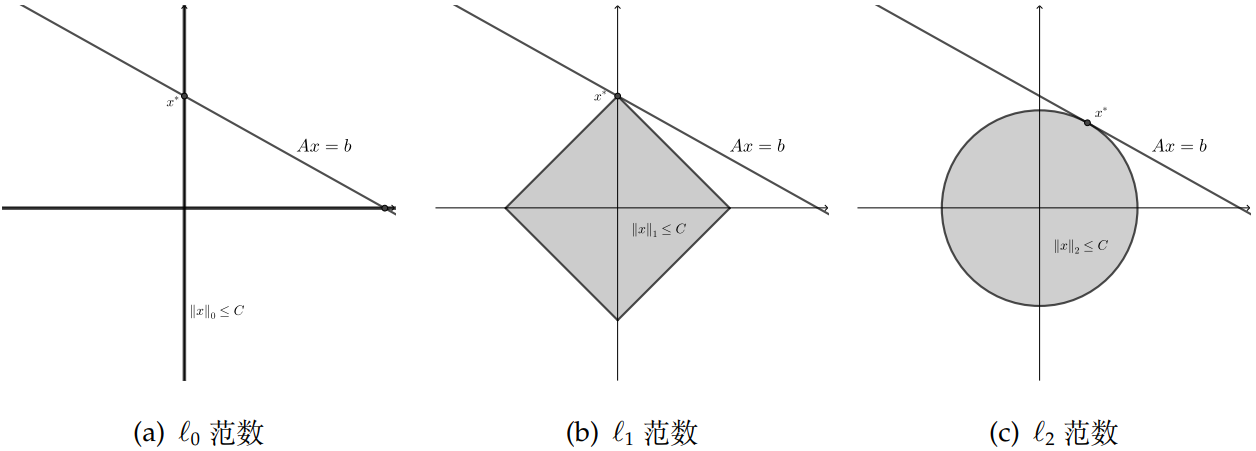
\includegraphics[width=.85\textwidth]{pics/norm optimize.png}
	\caption{$l_0, l_1, l_2$范数优化问题求解示意图}
	\label{fig:norm optimize}
\end{figure}
对$l_0$范数, $\{x | \|x\|_0 \leq 2\}$是全平面, 它自然与$A x = b$相交;$\{x | \|x\|_0 \leq 1\}$退化成两条直线即坐标轴, 此时问题的解就是$A x = b$与坐标轴的交点. 
\begin{itemize}
	\item 对$l_1$范数, 根据$C$不同, $\{x | \|x\|_1 \leq C\}$为一系列正方形, 这些正方形的顶点落在坐标轴上, $A x = b$与这些正方形的交点一般是在正方形的顶点即相交于坐标轴, 因此$l_1$范数的解有稀疏性
	
	\item 对$l_2$范数, 根据$C$不同, $\{x | \|x\|_1 \leq C\}$为一系列圆, 且圆有光滑的边界, 圆和$A x = b$的交点可以是圆上任何一点, 所以$l_2$范数优化问题一般不能保证解的稀疏性
\end{itemize}

注意: \tbc{red}{这里目标函数与约束函数相交一般是指相切, $\{x | \|x\|_p \leq C\}$可以看成一个广义的球体, 如果该球体与$A x = b$相交而不是相切, 那么一定存在一个更小的$C'$使$\|x\|_p$更小且与$A x = b$相切, 则$C'$成了比$C$更优的解, 故一般考虑相切. }

参考资料: 
\begin{itemize}
	\item《最优化: 建模、算法与理论》, 刘浩洋、户将、李勇锋、文再文编著, 第一章, 1.2
	\item \href{https://blog.csdn.net/red_stone1/article/details/80755144}{机器学习中 L1 和 L2 正则化的直观解释}
\end{itemize}


\subsection{Reparametrization}重参数化技术. 参考: \href{https://spaces.ac.cn/archives/6705}{漫谈重参数: 从正态分布到Gumbel Softmax}

\subsection{常用统计量}
\subsubsection{方差(Variance)} 一组数据的方差, 描述的是数据与它们的均值的离散程度, 衡量了这组数据的集中程度. 方差可以分为样本方差和总体方差: 
\begin{itemize}
	\item 样本方差: $S^2 = \frac{\sum_{i=1}^N(x_i - \bar{x})^2}{N-1}$, 其中$\bar{x}$是\textbf{样本均值}
	\item 总体方差: $\sigma^2 = \frac{\sum_{i=1}^N(x_i - \mu)^2}{N}$, 其中$\mu$是\textbf{总体均值}
\end{itemize}
\textbf{为什么不用要平方?}如果使用平均差($\frac{\sum_{i=1}^N |x_i - \bar{x}|}{N}$)来衡量一组数据的离散程度, 可能不能很好的体现数据的分散程度(参考: \href{https://www.shuxuele.com/data/standard-deviation.html#WhySquare}{为什么要求差的平方?}), 加上平方后可以放大偏离均值太远的数据的影响. 也许这有点像注意力机制, 在平均差中, $|x_i - \bar{x}|$的注意力值是$\frac{1}{N}$, 在方差中, $|x_i - \bar{x}|$的注意力值是$\frac{|x_i - \bar{x}|}{N}$, 这可以体现离均值越远的点对离散程度的贡献越大. 

\subsubsection{标准差(Standard Deviation)} 标准差的平方就是方差, 同理, 标准差也可以分为样本std.和总总体std.: 
\begin{itemize}
	\item 样本标准差: $S = \sqrt{S^2}$
	\item 总体标准差: $\sigma = \sqrt{\sigma^2}$
\end{itemize}

\subsubsection{T-statistic }


\subsubsection{p-value }

\subsubsection{t test、$\chi^2$检验}
$\chi^2$检验通常用于检验两个事件的独立性, 例如可以用于分析自变量与因变量之间的独立性. 如果$\chi^2$的值越大, 则说明二者之间的关联性越大. 

\subsection{数据的度量}
\subsubsection{定类变量}
即类别变量, 其值域是某个离散的类别. 能够对对象进行分类, 能够判断对象之间是否同类或异类, 如性别. \tbc{red}{不同类别之间没有大小关系}. 

\textbf{【可以分类( $=$ 和 $\neq$), 但不能排序】}

\subsubsection{定序变量}
定序变量的值不仅能够代表事物的分类, 还能代表事物按某种特性的排序, 但定序变量的值之间没有确切的间隔距离, \tbc{red}{只能排列出它们的顺序, 而不能反映出不同值之间的距离}, 即不能反映一个值比另一个值大多少或小多少. 如文化水平, 其取值可以是文盲、小学、中学、大学等, 值之间有顺序关系(如大学 $\textgreater$ 小学), 但不能反映不同文化程度之间的距离. 

\textbf{【可以分类( $=$ 和 $\neq$), 可以排序($\textgreater$ 和 $\textless$), 但不能($+$ 和 $-$ )】}

\subsubsection{定距变量}
定距变量的值之间\tbc{red}{可以比较大小, 两个值的差有实际意义}. 能确切测量值之间的高低、大小次序之间的距离, 因而具有加与减的数学特质. 但是, \tbc{red}{定距变量没有一个绝对的零点}, 不能乘除或倍数的形式来说明它们之间的关系. 例如华氏温度: 10、20、30, 30比20高10, 但华氏度30不是10的三倍热(\tbc{red}{0不是没有温度}). 

\textbf{【可以分类( $=$和 $\neq$ ), 可以排序($\textgreater$ 和 $\textless$), 可以($+$ 和 $-$ ), 但不能($\times$和 $\div$ )】}

\subsubsection{定比变量}
定比变量除了具有定距变量的特性外, 还具有一个真正的零点, 因而它具有乘与除(×、÷)的数学特质. 如A的体重是60kg, 而B的体重是30kg, 可以算出前者是后者的两倍重, 因为其零点是绝对的. 

\textbf{【可以分类( $=$和 $\neq$ ), 可以排序($\textgreater$ 和 $\textless$), 可以($+$ 和 $-$ ), 可以($\times$和 $\div$ )】}

以上四种变量类型的性质是逐渐继承的. 

参考: \href{https://blog.csdn.net/YYIverson/article/details/100068865}{【统计学】区分定类、定序、定距、定比变量!!}. 

\subsection{拉格朗日对偶性}
约束最优化中常用的一种方法. 利用拉格朗日对偶性(Lagrange duality)将原始问题转换为对偶问题, 通过求解对偶问题得到原始问题的解. 

\subsubsection{原始问题}假设$f(x), g_i(x), h_j(x)$是定义在$\mathbb{R}^n$的连续可微函数. 原始最优化问题为: 
\begin{align}
	\mathop{min}_{x \in \mathbb{R}^n}&\quad f(x) \nonumber \\
	s.t.&\quad g_i(x) \leqslant 0, i = 1, 2, ..., k \nonumber \\
		&\quad h_j(x) = 0, j = 1, 2, ..., l \nonumber
\end{align}

引进广义朗格朗日函数: 
$$
L(x, \alpha, \beta) = f(x) + \sum_{i=1}^k a_i g_i(x) + \sum_{i=j}^l \beta_j h_j(x)
$$
其中, $x \in \mathbb{R}^n$, $\alpha, \beta$是拉格朗日乘子, $\alpha_i \geqslant 0$. 将$L$看作$\alpha, \beta$的函数(固定$x$), 求其最大值, 即: 
$$
\mathop{max}_{\alpha, \beta:\alpha_i \geqslant 0} L(x, \alpha, \beta)
$$
注意, $\mathop{max}_{\alpha, \beta:\alpha_i \geqslant 0} L(x, \alpha, \beta)$表示固定$x$, $\alpha, \beta$作为变量来使$L$最大化, 此时再固定$\alpha, \beta$即可得到一个关于$x$的函数: 
$$
\theta_P (x) = \mathop{max}_{\alpha, \beta:\alpha_i \geqslant 0} L(x, \alpha, \beta)
$$
$P$表示原始问题. 分析一下$\theta_P$: 
\begin{myitemize}
	\item 当$x$违反原始约束, 即 $g_i(x) > 0$或$h_j(x) \neq 0$, 则可以很容易调整对应的$\alpha_i, \beta_j$使$\theta_P(x)$取得$+\infty$. (\textbf{$\alpha_i \geqslant 0$的原因})
	\item 当$x$满足原始约束时, 则有: 
	$$
	\theta_P(x) = \mathop{max}_{\alpha, \beta:\alpha_i \geqslant 0} L(x, \alpha, \beta) = f(x)
	$$
	考虑$f(x) + \sum_{i=1}^k a_i g_i(x) + \sum_{i=j}^l \beta_j h_j(x)$, 对于任意$x$(即固定$x$), 显然有$h_j(x) = 0$, 且$g_i(x) \leqslant 0$, 则$\mathop{max}_{\alpha, \beta:\alpha_i \geqslant 0} L(x, \alpha, \beta)$\textbf{肯定有$\alpha_i = 0$}, 所以, 
	$$
	\mathop{max}_{\alpha, \beta:\alpha_i \geqslant 0} L(x, \alpha, \beta) = f(x) + \sum_{i=1}^k 0 \cdot g_i(x) + \sum_{i=j}^l \beta_j h_j(x)
	$$
	即$\theta_P(x) = \mathop{max}_{\alpha, \beta:\alpha_i \geqslant 0} L(x, \alpha, \beta) = f(x)$
\end{myitemize}
因此, 
$$
\theta_P(z)= \begin{cases}f(x), & x\ satisfies\ subjects \\ +\infty, & \text { otherwise }\end{cases}
$$
所以$\theta_P(x)$的极小就等价于原始问题的解, 即: 
$$
\mathop{min}_{x} \theta_P(x) = \mathop{min}_{x} \mathop{max}_{\alpha, \beta: \alpha_i \geqslant 0} L(x, \alpha, \beta)
$$
因此, 原始不等式约束优化问题转化成了广义\textbf{拉格朗日的极小极大问题}, 定义原始问题的最优值: 
$$
p^* = \mathop{min}_{x} \theta_P(x)
$$

\subsubsection{对偶问题}
定义关于$\alpha, \beta$的函数, 
$$
\theta_D(\alpha, \beta) = \mathop{min}_{x} L(x, \alpha, \beta)
$$
$D$表示其为对偶问题, 其含义可与$\theta_P$类比. 考虑$\theta_D$的极大化, 即: 
$$
\mathop{max}_{\alpha, \beta: \alpha_i \geqslant 0} \theta_D(\alpha, \beta) = \mathop{max}_{\alpha, \beta: \alpha_i \geqslant 0} \mathop{min}_{x} L(x, \alpha, \beta)
$$
$\mathop{max}_{\alpha, \beta: \alpha_i \geqslant 0} \mathop{min}_{x} L(x, \alpha, \beta)$称为\textbf{拉格朗日函数的极大极小问题}. 将朗格朗日的极大极小问题转化为优化问题: 
\begin{align}
	\mathop{max}_{\alpha, \beta} \theta_D(\alpha, \beta)&\quad = \mathop{max}_{\alpha, \beta: \alpha_i \geqslant 0} \mathop{min}_{x} L(x, \alpha, \beta) \nonumber \\
	s.t.&\quad \alpha_i \geqslant 0, i = 1, 2, ..., k \nonumber
\end{align}
该问题称为原始问题的对偶问题, 定义对偶问题的最优值: 
$$
d^* = \mathop{max}_{\alpha, \beta: \alpha_i \geqslant 0} \theta_D(\alpha, \beta)
$$

\subsubsection{原始问题与对偶问题的关系}
若原始问题和对偶问题都有最优值, 那么二者的最优值有如下关系: 
$$
d^* = \mathop{max}_{\alpha, \beta: \alpha_i \geqslant 0} \mathop{min}_{x} L(x, \alpha, \beta) \leqslant \mathop{min}_{x} \mathop{max}_{\alpha, \beta: \alpha_i \geqslant 0} L(x, \alpha, \beta) = p^*
$$
\textbf{证明: }
\begin{quotation}
	$$
	\theta_D(\alpha, \beta) = \mathop{min}_{x} L(x, \alpha, \beta) \leqslant L(x, \alpha, \beta) \leqslant \mathop{max}_{\alpha, \beta: \alpha_i \geqslant 0} L(x, \alpha, \beta) = \theta_P(x)
	$$
	即, 
	$$
	\theta_D (\alpha, \beta) \leqslant \theta_P (x)
	$$
	即, 
	$$
	\mathop{max}_{\alpha, \beta:\alpha_i \geqslant 0} \theta_D (\alpha, \beta) \leqslant \mathop{min}_{x} \theta_P (x)
	$$
	得证. 
\end{quotation}
\textbf{推论: }
\begin{quotation}
	若$x^*, (\alpha^*, \beta^*)$分别是原始问题和对偶问题的\textbf{可行解}, 若$d^* = p^*$, 则$x^*, (\alpha^*, \beta^*)$分别是原始问题和对偶问题的\textbf{最优解}. 
\end{quotation} 
那什么样的条件才满足$d^* = p^*$呢?

\textbf{Karush-Kuhu-Tucker(KKT) 条件}\label{kkt}
\begin{quotation}
	对原始问题和对偶问题, 假设$f(x), g_i(x)$是凸函数, $h_j(x)$是仿射函数, 并且不等式约束$g_i(x) \leq 0$是\textbf{严格可行的}, 即存在$x$, 对所有$i$有$g_i(x) < 0$. 则$x^*, (\alpha^*, \beta^*)$分别是原始问题和对偶问题的解的充要条件是$x^*, (\alpha^*, \beta^*)$满足以下KKT条件: 
	\begin{align}\nonumber
		\nabla_x L(x^*, \alpha^*, \beta^*) &= 0 \nonumber \\
		\alpha_i^* g_i(x^*) &= 0, i = 1, 2, ..., k \nonumber \\
		g_i(x^*) &\leq 0, i = 1, 2, ..., k \nonumber \\
		\alpha_i^* &\geq 0, i = 1, 2, ..., k \nonumber \\ 
		h_j(x^*) &= 0, i = 1, 2, ..., l \nonumber 
	\end{align}
	
\end{quotation}

\subsection{Sequence Minimal Optimization(SMO)}\label{smo}
序列最小最优化算法, SMO是一种启发式算法, 通常用于求解凸二次规划问题. 

\subsection{正定核}\label{pdkf}
Positive definite kernel function. 一个核函数为正定核的充要条件: 
\begin{quotation}
	对任意$x_i \in \mathcal{R}, i = 1, 2, ..., m$ , $\kappa(x_i, x_j)$对应的Gram矩阵 $[\kappa(x_i, x_j)]_{m \times m}$是半正定矩阵. 
\end{quotation}

\subsubsection{常用核函数}
\begin{itemize}
	\item 多项式核: $\kappa(x, z) = (x \cdot z + 1)^p$
	\item 高斯核: $\kappa(x, z) = e^{- \frac{||x - z||^2}{2 \sigma^2}}$. 为啥说高斯核等于无穷维呢?因为 $e^x$ 这个函数进行展开的话有无穷维. 
\end{itemize}


\subsection{机器学习中常见的数据分布}
这里将介绍常见的一些分布, 主要通过这些分布的密度函数、分布函数来介绍, 以及其在机器学习/深度学习中的一些体现和应用. 
\subsubsection{Gaussian}高斯分布, 正态分布, 钟形分布. 
$$
f(x) = \frac{1}{\sqrt{2 \pi} \sigma} e^{- \frac{(x - \mu)^2 }{2 \sigma^2}}
$$
正态分布的两个参数为: $\mu, \sigma$, 分别表示正态分布的均值和标准差. 标准正态分布即 $\mu = 0, \sigma = 1$ 的正态分布. 

\subsubsection{Laplace}拉普拉斯分布. 
$$
f(x) = \frac{1}{2b} e^{- \frac{{|x - \mu|}}{b}}
$$


\subsection{变量之间的相关性检验}
在进行数据分析的时候, 如果要对自变量与因变量之间的关系进行分析, 或者说在多任务学习中, 分析不同任务之间的相关性时, 如何检验这种相关性是很重要的. 

\subsubsection{Person 相关系数}
即皮尔逊相关系数, 反应两个变量相似性的统计量, 衡量的是两个变量之间的\textbf{线性相关性}, 变化的趋势. 定义变量 $X, Y$ 的 Person 系数为: 
$$
\rho_{X, Y}=\frac{\operatorname{cov}(X, Y)}{\sigma_{X} \sigma_{Y}}=\frac{E[(X-E X)(Y-E Y)]}{\sigma_{X} \sigma_{Y}}=\frac{E(X Y)-E(X) E(Y)}{\sqrt{E\left(X^{2}\right)-E^{2}(X)} \sqrt{E\left(Y^{2}\right)-E^{2}(Y)}}
$$
其中 $\sigma$ 表示方差. 皮尔逊相关系数通常衡量的是两个实值变量之间的相关性, $\rho_{X, T} \in [-1, 1]$, 小于 0 表示负相关, 大于 0 表示正相关, 0 则表示二者不具备\textbf{线性}相关性. 注意, 不相关不等于独立. 当 $X, Y$ 是均值为 0 的变量时, 则有: 
$$
\rho_{X, Y}=\frac{E(X Y)}{\sqrt{E\left(X^{2}\right)} \sqrt{E\left(Y^{2}\right)}}=\frac{\frac{1}{N} \sum_{i=1}^{N} X_{i} Y_{i}}{\sqrt{\frac{1}{N} \sum_{i=1}^{N} X_{i}^{2}} \sqrt{\frac{1}{N} \sum_{i=1}^{N} Y_{i}^{2}}}=\frac{\sum_{i=1}^{N} X_{i} Y_{i}}{\sqrt{\sum_{i=1}^{N} X_{i}^{2}} \sqrt{\sum_{i=1}^{N} Y_{i}^{2}}}=\frac{\sum_{i=1}^{N} X_{i} Y_{i}}{\|X \mid\| Y \|}
$$
显然, 此时皮尔逊相关系数就成了两个向量的 $cosine$函数, 即余弦相似度, 再进一步, 如果 $X, Y$ 的模长为 1, 则皮尔徐相关系数 $\rho_{X, Y} = X \cdot Y$, 即成了向量的内积. 所以, 其实我们也可以反推出来, 向量的内积其实衡量的是向量的一种相似度, 一种未归一化的相似度. 

皮尔逊相关系数可以用来衡量两个用户之间的相似性, 例如以两个用户对物品的评分向量计算皮尔逊相关系数. 

\textbf{缺点}: 
\begin{itemize}
	\item 从皮尔逊相关系数的公式可以看出, 如果两个变量的配对的数据(即 $X, Y$ 都有值的数据, 在评分矩阵中体现为两个用户对同一个物品进行了评分你)很少时, 均值和方差的估计是不太准确的, 且只有一个配对时是无法计算皮尔逊相关系数的(因为方差为 0);
	\item 没有两个变量的配对的数目的影响, 即可能 $X, Y$ 之间的配对数量很大, 且值也比较接近, 但是如果 $X, Z$ 配对数量很小但评分基本一样, 则可能 $X, Y$ 的皮尔逊相关性会小于 $X, Z$ 的相关性, 这显然是不合理的;
	\item 要求变量的方差为 0, 即要求变量的值是取自一个方差不为零的分布(通常假设其来自正态分布), 其实从用户评分角度来看, 即要求用户的偏好是可以区分的;
	\item 对绝对值不敏感, 即 $X, Y$ 的趋势相似, 且值的分布也比较相似, $X, Z$ 的趋势相似但 $X$ 的平均值很大, $Z$ 的平均值很小, 用皮尔逊相系数衡量的话, 可能 $X, Z$ 之间更相似. 在推荐中, 可能优的用户习惯给低分, 有的用户习惯给高分; 
\end{itemize}

\subsubsection{Spearman 秩相关系数}
Spearman 秩相关系数是一种无参数(与分布无关)检验方法, 用于度量变量之间联系的强弱, \textbf{是否存在单调性关系}. 在没有重复数据的情况下, 如果一个变量是另外一个变量的严格单调函数, 则Spearman秩相关系数就是 +1 或 -1, 称变量完全 Spearman 秩相关. 注意\textbf{与 Pearson 完全相关的区别}: 只有当两变量存在线性关系时, Pearson 相关系数才为 +1 或 -1; 而且, 由于 Spearman 是先对数据进行排序再进行计算, 因此对错误数据和异常值更鲁棒, Person 则不然.

将 $X, Y$ 两个变量的取值看作序列, 计算 $x_i$ 在 $X$ 中的顺序(秩), 对于 $Y$ 计算相同的值, 对于一对 $(x_i, y_i)$ 而言, 秩差 $d_i$ 为 $x_i, y_i$ 的秩的差, 则斯皮尔曼系数为: 
$$
\rho_{s} = 1 - \frac{6 \sum_{i=1}^N d_i^2}{N(N^2 - 1)}
$$
显然, 斯皮尔曼系数不仅可以度量变量之间的线性和非线性相关性, 如 $y = x^2, x > 0$, 用皮尔逊系数度量则为不相关的, 但是在斯皮尔曼系数下可以算得二者得相关性是 1. 其实, 虽然斯皮尔曼不要求变量是来自某个分布得, 但是可以看出它还是要求变量得值是可以比较得, 否则秩就没有意义了. 且要处理变量中存在重复值得情况, 即在 $X$ 或 $Y$ 中存在重复值时该如何赋予秩. 

当然, 对于不同的变量类型, 有不同得检验方法, 具体可以参见: \href{https://zhuanlan.zhihu.com/p/396580986}{相关分析最全总结}、\href{https://zhuanlan.zhihu.com/p/94070722}{要做相关性分析, 该如何选择正确的统计方法?}

\subsection{Jacobean, Hessian}
雅可比矩阵指的是函数对输入的一阶导矩阵, 假设有函数 $f: \mathbb{R}^m \longmapsto \mathbb{{R}^n}$. $f$ 的每一个输出可以用于一个单输出的函数表示$y_i(x_1, x_2, \dots, x_m),\ \ i=1\cdots n$. 雅可比矩阵即 $f$ 对输入的一阶导:

$$
\nabla f = \frac{\partial f}{\partial x} = \left[\begin{array}{ccc}
	\frac{\partial y_{1}}{\partial x_{1}} & \cdots & \frac{\partial y_{1}}{\partial x_{n}} \\
	\vdots & \cdots & \vdots \\
	\frac{\partial y_{m}}{\partial x_{1}} & \cdots & \frac{\partial y_{m}}{\partial x_{n}}
\end{array}\right]
$$

可以看到雅可比矩阵是一个 $\mathbb{R}^{m \times n}$ 的矩阵, 每一行是一个输出对输入向量的一阶导.

与雅可比矩阵不同, 海森矩阵是一个单输出的函数对输入的二阶导的矩阵. 假设有函数 $g: \mathbb{R}^n \longmapsto \mathbb{R}$. 则其海森矩阵为:

$$
\nabla^2 g = \frac{\partial^2 g}{\partial x^2}=\left[\begin{array}{ccc}
	\frac{\partial^{2} g}{\partial x_{1}^{2}} & \cdots & \frac{\partial^{2} g}{\partial x_{1} \partial x_{n}} \\
	\vdots & \ddots & \vdots \\
	\frac{\partial^{2} g}{\partial x_{n} \partial x_{1}} & \cdots & \frac{\partial^{2} g}{\partial x_{n}^{2}}
\end{array}\right]
$$

可以看大, 海森矩阵是一个 $\mathbb{R}^{n \times n}$ 的矩阵. 如果把 $g$ 的一阶导定义为一个函数 $\nabla g$, 则 $g$ 的海森矩阵就是 $\nabla g$ 的雅可比矩阵.

\subsection{指数移动平均}
指数移动平均在深度学习的梯度下降优化算法中出现的频率很高. 

\subsection{牛顿法}
牛顿法是一种比较常用的优化算法, 与常见的梯度下降不同, 牛顿法是一种二阶的优化算法. 其基本思想是利用迭代点处的一阶导数 (梯度) 和二阶导数 (Hessian矩阵) 对目标函数进行二次函数近似, 然后把二次模型的极小点作为新的迭代点, 并不断重复这一过程, 直至求得满足精度的近似极小值. 牛顿法的速度快, 而且能高度逼近最优值. 牛顿法分为基本的牛顿法和全局牛顿法.

假设待优化的目标函数为 $f(x)$, 通常优化问题可以转化为求梯度为 0 的点, 即 $f^{\prime}(x) = 0$. 将 $f(x)$ 在 $x_k$ 处进行泰勒展开到二阶:

$$
f(x)=f\left(x_{k}\right)+f^{\prime}\left(x_{k}\right)\left(x-x_{k}\right)+\frac{1}{2} f^{\prime \prime}\left(x_{k}\right)\left(x-x_{k}\right)^{2}
$$

对上式进行求导并令其等于 0 则得到:

$$
f^{\prime}\left(x_{k}\right)+f^{\prime \prime}\left(x_{k}\right)\left(x-x_{k}\right)=0
$$

可以得到:

$$
x=x_{k}-\frac{f^{\prime}\left(x_{k}\right)}{f^{\prime \prime}\left(x_{k}\right)}
$$

其中 $x_k$ 就是上一次得到的迭代点, $x$ 就是我们新得到的迭代点 $x_{k+1}$. 这个的 $f$ 是一个一元函数, 若 $f$ 是多元函数, 则 $x$ 的迭代式为:

$$
x_{k+1} = x_k - H^{-1}_k g_k
$$

其中 $g_k$ 是 $f$ 的一阶导在 $x_k$ 的取值, $H_k$ 是 $f$ 的海森矩阵在 $x_k$ 的取值.

牛顿法的\textbf{特点}: 1) 收敛速度快; 2) 对起始迭代点敏感, 如果初始点离最优点很远, 可能会不收敛; 3) 需要计算海森矩阵的逆, 但可能该矩阵是不可逆的且求逆的计算量很大 (拟牛顿法就是针对这个问题提出来的); 

\subsection{最小二乘法}
Least Square Method, 也叫最小平方法. 见名知意, 基本思想就是: 找到一组参数, 使模型的预测值与目标值的\textbf{误差的平方和最小}, 即:
$$
L = \sum_{i=1}^n (y_i - f(x_i))^2
$$

其中, $f(x) = w \cdot x + b$. 最小二乘法的求解, 即求解 $w$ 可以通过矩阵解法也可以通过梯度下降法, 这里就不再赘述了. 注意, 最小二乘法中有一个假设: \textcolor{red}{误差的分布是正态分布}.

\subsection{rand5 和 rand7 的转换}
之前听到这种随机数生成的问题以为还是挺简单的, 直到最近看到一个关于 rand5 和 rand7 之间转换的问题, 才发现自己之前想的太简单了. 进行正确的转换, 有两个条件要满足: 1) 取值范围要正确; 2) \textbf{转换后, 生成每个值是等概率的}. 其中第二条是我以前忽视的, 现在一想, 这个问题还是有点意思的. 先定义一下 randa: 随机整数数生成函数, 可以等概率地随机生成 $[1, a]$ 中的值. 

\textbf{先看一下如何用 rand7 生成rand5}. 

\begin{python}
	def rand5():
		x = 1<<31
		while x > 5:
			x = rand7()
		
		return x
\end{python}

首先, 这肯定是能够生成 $[1, 5]$ 范围内地数的, 但是是等概率的吗? 算一算生成 1 的概率:
$$
\begin{aligned}
	P(x=1) &= \frac{1}{7} + \frac{2}{7} \times \frac{1}{7 } + (\frac{2}{7})^2 \times \frac{1}{7} + \dots + (\frac{2}{7})^n \times \frac{1}{7} \\
		   &= \frac{1}{5}
\end{aligned}
$$

上式分别表示第一次就生成 1 的该率, 第二次, ... 第 n 次生成 1 的概率. 所以这个方法是可行的. 所以, 如果有两个随机数生成器 randa 和 randb. 如果用 randa 生成 randb 且 $a > b$, 那么直接按照上述的方法做就可以了.

\textbf{那怎么用 rand5 生成 rand7 呢?}
如果我用 rand5 + rand3 - 1 生成 rand7, 这样貌似生成了 $[1, 7]$ 之间的数, 但是这是等概率的吗? 并不是! 生成 1 只有一种情况, 而生成 2 则有 2 中, 生成 4 则更大. 我们利用上一步的方法, 先用 rand5 生成一个更大的随机数生成器, 例如 rand25 = 5 * (rand5 - 1) + rand5. 检查一下是否满足那俩条件. 首先 5 * (rand5 - 1) 可以等概率地生成 0, 5, 10, 15, 20. 加上 rand5 后可以生成 $[1, 25]$ 且每个数只有一种情况. 因此我们成过得到了一个 rand25. 还愣着干嘛, 直接套用上述地方法生成 rand7 啊!

\begin{python}
	def rand7():
		x = 1<<31
		while x > 7:
			x = 5 * (rand5() - 1) + rand5()
	
	return x
\end{python}

问题看似解决了, 但是 7 和 25 之间还有很长一段距离, 生成地很多数据都会被抛弃掉, 浪费时间. 那怎么优化呢? 为了让抛弃地数尽量少, 即让上述代码里地 \mintinline{python}{while} 循环尽快的跳出, 可以生成 randc, c 是最接近 25 的 7 的倍数, 即 21, 再根据 rand21 生成 rand7, 此时只要对 7 取余再加 1 就行了, 显然这是满足条件的:

\begin{python}
	def rand7():
		x = 1<<31
		while x > 21:
			x = 5 * (rand5() - 1) + rand5()
	
	return x % 7 + 1
\end{python}

\textbf{对上述问题进行一个泛化}. 用 randa 生成 randb 且 $a < b$ 怎么办?
\begin{enumerate}
	\item 构造 rand$a^2$ = a * (randa - 1) + randa, 生成 $[1, a^2]$ 的数, 如果 $a^2 < b$, 则继续构造 rand$a^3$, 直至得到 rand$a^k$ 使 $a^k > k$, 记为 randA;
	
	\item 用 randA 来构造 randb, 构造代码如下:
	  \begin{python}
	  	def randb():
		  	x = 1<<31
		  	while x > b * A // b:
		  		x = randA()
	  	
	  	return x % 7 + 1
	  \end{python}
  	注意 \mintinline{python}{while} 的判断条件 $b * A // b$, 即找到小于 A 的最大的 b 的倍数.
\end{enumerate}

感谢博客: \href{https://blog.csdn.net/u010025211/article/details/49668017}{使用rand5()生成rand7()}.

\subsection{神经网络中的求导}
参考资料: \href{https://web.stanford.edu/class/cs224n/readings/gradient-notes.pdf}{Computing Neural Network Gradients}.